\documentclass{article}

\usepackage{tabularx}
\usepackage{booktabs}
\usepackage{hyperref}
\usepackage{graphicx}
\usepackage{svg}


\title{Problem Statement and Goals\\\progname}

\author{\authname}

\date{}

%% Comments

\usepackage{color}

\newif\ifcomments\commentstrue %displays comments
%\newif\ifcomments\commentsfalse %so that comments do not display

\ifcomments
\newcommand{\authornote}[3]{\textcolor{#1}{[#3 ---#2]}}
\newcommand{\todo}[1]{\textcolor{red}{[TODO: #1]}}
\newcommand{\note}[1]{\textcolor{red}{[#1 \#NOTE]}}
\else
\newcommand{\authornote}[3]{}
\newcommand{\todo}[1]{}
\fi

\newcommand{\wss}[1]{\authornote{blue}{SS}{#1}} 
\newcommand{\plt}[1]{\authornote{magenta}{TPLT}{#1}} %For explanation of the template
\newcommand{\an}[1]{\authornote{cyan}{Author}{#1}}


%% Common Parts


\newcommand{\progname}{Agolearn} % PUT YOUR PROGRAM NAME HERE
\newcommand{\thisproject}{\progname}
\newcommand{\authname}{Team 1, Agonaught(s)
\\ Yiding Li} % AUTHOR NAMES                  

\usepackage{hyperref}
    \hypersetup{colorlinks=true, linkcolor=blue, citecolor=blue, filecolor=blue,
                urlcolor=blue, unicode=false}
    \urlstyle{same}
                                


\begin{document}

\maketitle

\begin{table}[hp]
\caption{Revision History} \label{TblRevisionHistory}
\begin{tabularx}{\textwidth}{llX}
\toprule
\textbf{Date} & \textbf{Developer(s)} & \textbf{Change}\\
\midrule
2024-01-15 & Yiding Li & First Draft\\
2024-01-16 & Yiding Li & Add and resolve TODO items
\begin{enumerate}
    \item Clarify inputs
    \item Clarify goals
    \item Refine stakeholders
    \item Fix an erroneous figure and its caption
    \item Resolve TODO item on adding references
\end{enumerate}
\\
2024-01-15 & Yiding Li & Return \textbf{Motivation} to \textbf{Problem}: describe "what it does", not "what it is".\\
\bottomrule
\end{tabularx}
\end{table}

\section{Problem Statement}

% \wss{You should check your problem statement with the
% \href{https://github.com/smiths/capTemplate/blob/main/docs/Checklists/ProbState-Checklist.pdf}
% {problem statement checklist}.}
% \wss{You can change the section headings, as long as you include the required information.}

\subsection{Motivation}

This project seeks to implement an evolutionary optimizer for arbtrary real-valued functions and higher-ordered functions.

While \hyperref[sec:evalg]{evolutionary algorithms} lack the efficiency of traditional optimization algorithms, they lend well to solving poorly understood, dynamic, or black-box problems. As such, usage of evolutionary algorithms is key to imeplemting this project. \hyperref[sec:genalg]{Generic programming algorithms}, in particular, make it possible to build functions that optimize higher-order functions.

\begin{figure}[h]
    \caption{Input and output of a genetic programming algorithm}
    \includegraphics[width=\textwidth]{example\_learn.png}
    \centering
\end{figure}

\subsection{Inputs and Outputs}


\subsubsection{Optimizing real-valued functions}
\textbf{Input}:
\begin{enumerate}
    \item A real-valued function.
    \item Parameters that control the evolutionary process. Examples are: (a) choices of evolutoinary operators, (b) number of episodes, and (c) the length of each episode or truncation conditions.
\end{enumerate}
\textbf{Output}: A real vector that optimizes the given real-valued function.

\subsubsection{Optimizing higher-ordered functions}
\textbf{Input}:
\begin{enumerate}
    \item A higher-order function.
    \item Parameters that control how solutions are generated. Examples are: (a) node functions, (b) tree depth, and (c) node count.
    \item Parameters that control the evolutionary process. Examples are: (a) choices of evolutoinary operators, (b) number of episodes, and (c) the length of each episode or truncation conditions.
\end{enumerate}
\textbf{Output}: A function that optimizes the given higher-order function.

\subsection{Stakeholders}
This project can be used by anyone who seeks to optimize an objective function. It should be especially suited for derivative-free functions.

\section{Goals}
\begin{itemize}
    \item Optimize against real-valued functions
    \item Optimize against higher-order functions
\end{itemize}

\section{Stretch Goals}

\begin{itemize}
    \item Optimize against an objective function of functions (genetic programs)
    \item Implement multi-processing to speed up computation (in reference to frameworks such as \href{https://deap.readthedocs.io/en/master/}{Deap})
\end{itemize}
\section{Appendix}

\subsection{Evolutionary Algorithms}
\label{sec:evalg}
\textbf{Evolutionary algorithms} (\textbf{EA}) are optimization algorithms that draw on the evolutionary process. An EA begins with an initial population, then iteratively improves the population through generations by applying various \hyperref[sec:evop]{evolutionary operators}.

\subsection{Evolutionary Operators}
\label{sec:evop}
\textbf{Evolutionary operators} divide into \textbf{parent selectors}, \textbf{variators}, and \textbf{survivor selectors}. These operators emulate events in an evolutionary process:

\begin{itemize}
    \item \textbf{Parent selectors} select from the population to form the parent pool.
    \item \textbf{Variators} act on the parent pool to produce a pool of offsprings. An offspring may inherit traits from parents (by crossover) or posess novel traits (by mutation).
    \item \textbf{Survivor selectors} select from the offspring pool to form the population for the next generation.
\end{itemize}

\begin{figure}[h]
    \caption{Stages and operators in an evolutionary episode}
    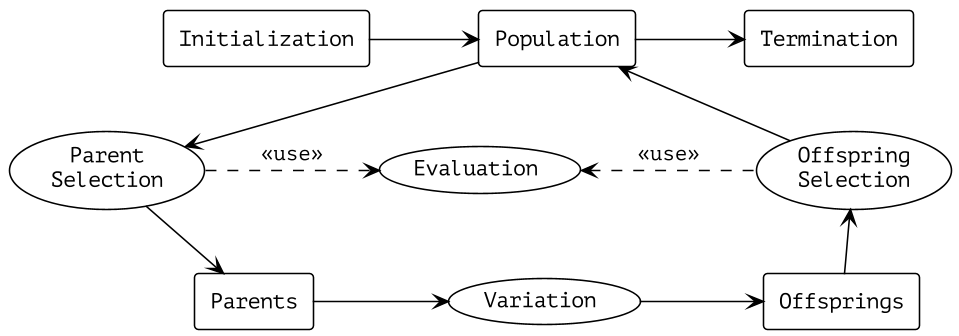
\includegraphics[width=\textwidth]{ramen}    
    \centering
\end{figure}

\subsection{Genetic Programming}
\label{sec:genalg}
\textbf{Genetic programming} (\textbf{GA}) algorithms are evolutionary algorithms that evolve with programs. That is, such algorithms evolve \textit{functions} against an higher-order objective function that takes functions as input. Genetic algorithms can evolve agents that behave well in a particular environment (e.g. \href{https://www.mdpi.com/2227-7390/11/13/2931}{a bipedal walker}) or construct mathematical models (e.g. \href{https://link.springer.com/article/10.1007/s11831-023-09922-z}{symbolic regression})



\end{document}